\documentclass{article}

% if you need to pass options to natbib, use, e.g.:
% \PassOptionsToPackage{numbers, compress}{natbib}
% before loading nips_2017
%
% to avoid loading the natbib package, add option nonatbib:
% \usepackage[nonatbib]{nips_2017}

\usepackage[nonatbib]{nips_2017}

% to compile a camera-ready version, add the [final] option, e.g.:
% \usepackage[final]{nips_2017}

\usepackage[utf8]{inputenc} % allow utf-8 input
\usepackage[T1]{fontenc}    % use 8-bit T1 fonts
\usepackage{hyperref}       % hyperlinks
\usepackage{url}            % simple URL typesetting
\usepackage{booktabs}       % professional-quality tables
\usepackage{amsfonts}       % blackboard math symbols
\usepackage{nicefrac}       % compact symbols for 1/2, etc.
\usepackage{microtype}      % microtypography
\usepackage{mathtools}
\usepackage{textcomp}
\usepackage{amsmath}
\usepackage{amsthm}
\usepackage{lmodern}
\usepackage{amssymb}
\usepackage{amsfonts}
\usepackage{amsxtra}
\usepackage[babel,theoremfont]{newpxtext}
\usepackage[bigdelims,nosymbolsc]{newpxmath}
\usepackage{bm}
\usepackage{mathdots}
\usepackage[usenames]{xcolor}
\usepackage[defblank,neveradjust]{paralist}
\usepackage[shortlabels]{enumitem}
\usepackage[british]{babel}
\selectlanguage{british}
\newcommand*{\langfrench}{\foreignlanguage{french}}
\newcommand*{\langgerman}{\foreignlanguage{german}}
\newcommand*{\langitalian}{\foreignlanguage{italian}}
\newcommand*{\langswedish}{\foreignlanguage{swedish}}
\newcommand*{\langlatin}{\foreignlanguage{latin}}
\newcommand*{\langnohyph}{\foreignlanguage{nohyphenation}}
\newcommand*{\latin}[1]{\langlatin{#1}}
\newcommand*{\french}[1]{\emph{\langfrench{#1}}}
\newcommand*{\german}[1]{\emph{\langgerman{#1}}}
\usepackage[autostyle=false,autopunct=false,english=british]{csquotes}
\setquotestyle{american}

\usepackage[%
backend=biber,%
mcite,%
subentry,%
citestyle=numeric-comp,%
bibstyle=numericbringhurst,%
%bibstyle=chem-biochem,%
autopunct=false,%
sorting=none,%
sortcites=false,%
%style=verbose,%
natbib=false,
maxnames=8,minnames=8,% maxnames=2,minnames=1,
giveninits=true,%
block=space,%
hyperref=true,%
defernumbers=false,%
%refsegment=chapter,%
useprefix=true%
,language=british%
]{biblatex}
\DeclareDelimFormat{multicitedelim}{\addsemicolon\space}
\DeclareDelimFormat{postnotedelim}{\space}
\addbibresource{portamanabib.bib}
\renewcommand{\bibfont}{\footnotesize}
\defbibheading{bibliography}[\bibname]{\section*{#1}\addcontentsline{toc}{section}{#1}%\markboth{#1}{#1}
}
\renewcommand*{\finalnamedelim}{, }
\setcounter{biburlnumpenalty}{1}
\setcounter{biburlucpenalty}{0}
\setcounter{biburllcpenalty}{1}
\newcommand*{\citep}{\parencites}
\newcommand*{\citey}{\parencites*}
\renewcommand{\cite}{\citep}
\providecommand{\href}[2]{#2}
\providecommand{\eprint}[2]{\texttt{\href{#1}{#2}}}
%\renewcommand{\eprint}[2]{\texttt{\href{#1#2}{#2}}}

%\DeclareBibliographyCategory{extras}

\def\arxivp{}
\def\mparcp{}
\def\philscip{}
\def\biorxivp{}

\providecommand*{\urlalt}{\href}

\newcommand*{\arxivsi}{\texttt{arXiv} eprints available at \url{http://arxiv.org/}.\\}
\newcommand*{\mparcsi}{\texttt{mp\_arc} eprints available at \url{http://www.ma.utexas.edu/mp_arc/}.\\}
\newcommand*{\philscisi}{\texttt{philsci} eprints available at \url{http://philsci-archive.pitt.edu/}.\\}
\newcommand*{\biorxivsi}{\texttt{bioRxiv} eprints available at \url{http://biorxiv.org/}.\\}

\newcommand*{\arxiveprint}[1]{\global\def\arxivp{\arxivsi}%\citeauthor{0arxivcite}\addtocategory{ifarchcit}{0arxivcite}%eprint
\texttt{\urlalt{http://arxiv.org/abs/#1}{arXiv:\bd #1}}%
%\texttt{\href{http://arxiv.org/abs/#1}{\protect\url{arXiv:#1}}}%
%\renewcommand{\arxivnote}{\texttt{arXiv} eprints available at \url{http://arxiv.org/}.}
}

\newcommand*{\mparceprint}[1]{\global\def\mparcp{\mparcsi}%\citeauthor{0mparccite}\addtocategory{ifarchcit}{0mparccite}%eprint
\texttt{\urlalt{http://www.ma.utexas.edu/mp_arc-bin/mpa?yn=#1}{mp\_arc:\bd #1}}%
%\texttt{\href{http://www.ma.utexas.edu/mp_arc-bin/mpa?yn=#1}{\protect\url{mp_arc:#1}}}%
%\providecommand{\mparcnote}{\texttt{mp_arc} eprints available at \url{http://www.ma.utexas.edu/mp_arc/}.}
}

\newcommand*{\philscieprint}[1]{\global\def\philscip{\philscisi}%\citeauthor{0philscicite}\addtocategory{ifarchcit}{0philscicite}%eprint
\texttt{\urlalt{http://philsci-archive.pitt.edu/archive/#1}{PhilSci:\bd #1}}%
%\texttt{\href{http://philsci-archive.pitt.edu/archive/#1}{\protect\url{PhilSci:#1}}}%
%\providecommand{\mparcnote}{\texttt{philsci} eprints available at \url{http://philsci-archive.pitt.edu/}.}
}

\newcommand*{\biorxiveprint}[1]{\global\def\biorxivp{\biorxivsi}%\citeauthor{0arxivcite}\addtocategory{ifarchcit}{0arxivcite}%eprint
\texttt{\urlalt{http://biorxiv.org/content/early/#1}{bioRxiv:\bd #1}}%
%\texttt{\href{http://arxiv.org/abs/#1}{\protect\url{arXiv:#1}}}%
%\renewcommand{\arxivnote}{\texttt{arXiv} eprints available at \url{http://arxiv.org/}.}
}

\newtheoremstyle{innote}%
{\parsep}%
{\parsep}%
{\footnotesize}%
{}%
{}%
{}%
{0pt}%
{}%
\theoremstyle{innote}
\newtheorem*{innote}{}


\title{Inferences from a network to a subnetwork, and vice versa, under an assumption of symmetry}

% The \author macro works with any number of authors. There are two
% commands used to separate the names and addresses of multiple
% authors: \And and \AND.
%
% Using \And between authors leaves it to LaTeX to determine where to
% break the lines. Using \AND forces a line break at that point. So,
% if LaTeX puts 3 of 4 authors names on the first line, and the last
% on the second line, try using \AND instead of \And before the third
% author name.

\author{
  David S.~Hippocampus\thanks{Use footnote for providing further
    information about author (webpage, alternative
    address)---\emph{not} for acknowledging funding agencies.} \\
  Department of Computer Science\\
  Cranberry-Lemon University\\
  Pittsburgh, PA 15213 \\
  \texttt{hippo@cs.cranberry-lemon.edu} \\
  %% examples of more authors
  %% \And
  %% Coauthor \\
  %% Affiliation \\
  %% Address \\
  %% \texttt{email} \\
  %% \AND
  %% Coauthor \\
  %% Affiliation \\
  %% Address \\
  %% \texttt{email} \\
  %% \And
  %% Coauthor \\
  %% Affiliation \\
  %% Address \\
  %% \texttt{email} \\
  %% \And
  %% Coauthor \\
  %% Affiliation \\
  %% Address \\
  %% \texttt{email} \\
}



%@@@@@@@@@@@@@@@@@@@@@@@ new commands @@@@@@@@@@@@@@@@@@@@@

\providecommand{\defaultlists}{}
%\newcommand*{\av}{\widebar} %pop average
\newcommand*{\av}{\overline} %pop average
\newcommand*{\sav}{\widehat} %subpop average

\newcommand*{\yx}{\bm{x}}%subpop state
\newcommand*{\yxs}{\sav{\yx}}%subpop av state
\newcommand*{\yX}{\bm{X}}%pop state
\newcommand*{\yXf}{\av{\yX}}%pop av state
\newcommand*{\yr}{\bm{r}}%subpop value
\newcommand*{\yrs}{\sav{\yr}}%subpop av value
\newcommand*{\yR}{\bm{R}}%pop value
\newcommand*{\yRf}{\av{\yR}}%pop av value
%conditional assumptions
\newcommand*{\yH}{\varEta}
\newcommand*{\yD}{\varDelta}
\newcommand*{\yHa}{\varEta'}
\newcommand*{\yHb}{\varEta''}
%Lagr multipliers
\newcommand*{\yL}{\varLambda}
\newcommand*{\yl}{\lambda}
\newcommand*{\yk}{\kappa}
%entropies
\newcommand*{\ysh}{H}
\newcommand*{\ybu}{H_{\text{B}}}

\newcommand*{\prop}[1]{`#1'}
\DeclarePairedDelimiter\set{\{}{\}}
\newcommand*{\amp}{\&}

%Latin abbrev.
\newcommand*{\vs}{{vs.}}
\newcommand*{\etc}{{etc.}}
\newcommand*{\ie}{{i.e.}}
\newcommand*{\ca}{{c.}}
\newcommand*{\Ie}{{I.e.}}
\newcommand*{\Eg}{{E.g.}}
\newcommand*{\eg}{{e.g.}}
\newcommand*{\viz}{{viz}}
\newcommand*{\cf}{{cf.}}
\newcommand*{\Cf}{{Cf.}}
\newcommand*{\vd}{{v.}}
\newcommand*{\Vd}{{V.}}
\newcommand*{\etal}{{et al.}}
\newcommand*{\etsim}{{et sim.}}
\newcommand*{\ibid}{{ibid.}}
\newcommand*{\sic}{{sic}}
%%%%%%%%%%%%%%%%%%%%%%%%%%%%%%%%%%%%%%%%%%%%%%



\newcommand*{\defd}{\coloneqq}
\newcommand*{\defs}{\eqqcolon}
\newcommand*{\Land}{\bigwedge}
\newcommand*{\Lor}{\bigvee}
\newcommand*{\lland}{\mathbin{\ \land\ }}
\newcommand*{\llor}{\mathbin{\ \lor\ }}
\newcommand*{\lonlyif}{\mathbin{\Rightarrow}}%implies
\newcommand*{\limplies}{\mathbin{\Rightarrow}}%implies
\newcommand*{\mimplies}{\Rightarrow}%implies
\newcommand*{\liff}{\mathbin{\Leftrightarrow}}%if and only if
%\newcommand*{\lequal}{=}%identical propositions
%\newcommand*{\ldef}{\defd}%equivalent by def.
%\newcommand*{\ldefin}{\stackrel{_\text{def}}{\Longleftrightarrow}}
\newcommand*{\cond}%{|}%
{\mathpunct{|}}%conditional sign (in probabilities)
\newcommand*{\lcond}%{|}%
{\mathpunct{|\ }}%conditional sign (in probabilities)
\newcommand*{\bigcond}{\mathpunct{\big|}}%conditional sign (in probabilities)
\newcommand*{\lbigcond}{\mathpunct{\big|\ }}%conditional sign (in probabilities)
\newcommand*{\suchthat}{\mid}%{\mathpunct{|}}%such that (eg in sets)
\newcommand*{\bigst}{\mathpunct{\big|}}%such that (eg in sets)
\newcommand*{\with}{\colon}%with (list of indices)
\newcommand*{\mul}{\times}%multiplication
\newcommand*{\inn}{\cdot}%inner product
\newcommand*{\dotv}{\mathord{\,\cdot\,}}%variable place
%\newcommand*{\cross}{\times}%vector product
%\newcommand*{\cart}{\times}%cartesian product
\newcommand*{\comp}{\circ}%composition of functions
%\DeclareMathOperator{\conv}{conv}%convex hull
\DeclareMathOperator*{\argmax}{arg\,max}%convex hull
%\newcommand*{\convl}{*}%convolution
\newcommand*{\con}{\mathbin{:}}%scal prod of tensors
%\newcommand*{\tpro}{\otimes}%tens prod
\newcommand*{\equi}{\sim}%equivalent to
\newcommand*{\corr}{\mathrel{\hat{=}}}%corresponds to
\providecommand{\varparallel}{\ensuremath{\mathbin{/\mkern-7mu/}}}%parallel (tentative symbol)
%\newcommand*{\paral}{\varparallel}%parallel (tentative symbol)
%\newcommand*{\asym}{\simeq}%asymptotically equal to
%\newcommand*{\prop}{\simeq}%asymptotically equal to
\renewcommand{\le}{\leqslant}%less or equal
\renewcommand{\ge}{\geqslant}%greater or equal

\newcommand*{\vect}[1]{\bm{#1}}%vectors
%probability
\DeclareMathOperator{\pr}{P}%probability
\newcommand*{\pf}{\mathrm{p}}%probability
%\DeclareMathOperator{\G}{\Gamma}%probability density
\newcommand*{\p}{\mathrm{P}}%probability
\newcommand*{\tf}{\mathrm{T}}%probability
\renewcommand*{\|}{\cond}
\newcommand*{\+}{\lor}
\newcommand*{\un}{\;\mathrm}
%\newcommand*{\comma}{\mathord{.}}% space
%\newcommand*{\uni}[1]{\textnormal{#1}}% unity
%\newcommand*{\tim}{\cdot}% multipl
%\newcommand*{\per}{/}% per
%Sections and theorem-like environments
\newcommand*{\sect}{\S}% Sect.~
\newcommand*{\sects}{\S\S}% Sect.~
\newcommand*{\chap}{ch.}%
\newcommand*{\chaps}{chs}%
\newcommand*{\fn}{fn}%
\newcommand*{\eqn}{eq.}%
\newcommand*{\eqns}{eqs}%
\newcommand*{\fig}{fig.}%
\newcommand*{\figs}{figs}%

%%%%%%%%%%%%%%%%%%%%%%%%%%%%%%%%%%%%%%%%%%%%%%
\newcommand*{\ordm}[2]{(#1,#2)}%matrix order
%\DeclareMathOperator{\rank}{rank}%rank
%\DeclareMathOperator{\range}{range}%range
\newcommand*{\id}{\mathte{I}}%id matrix
\newcommand*{\nbd}{\nobreakdash}%
\newcommand*{\bd}{\hspace{0pt}}%
\def\hy{-\penalty0\hskip0pt\relax}

\newcommand*{\labelbis}[1]{\tag*{(\ref{#1})$_\text{r}$}}
\newcommand*{\mathbox}[2][.8]{\parbox[t]{#1\columnwidth}{#2}}
\newcommand*{\zerob}[1]{\makebox[0pt][l]{#1}}

\newcommand*{\rtext}[1]{\mathrel{\text{#1}}}



\let\varAlpha A
\newcommand*{\Beta}{\mathrm{B}}
\let\varBeta B
\newcommand*{\Epsilon}{\mathrm{E}}
\let\varEpsilon E
\newcommand*{\Zeta}{\mathrm{Z}}
\let\varZeta Z
\newcommand*{\Eta}{\mathrm{H}}
\let\varEta H
\newcommand*{\Iota}{\mathrm{I}}
\let\varIota I
\newcommand*{\Kappa}{\mathrm{K}}
\let\varKappa K
\newcommand*{\Mu}{\mathrm{M}}
\let\varMu M
\newcommand*{\Nu}{\mathrm{N}}
\let\varNu N
\newcommand*{\Omicron}{\mathrm{O}}
\let\varOmicron O
\newcommand*{\Rho}{\mathrm{P}}
\let\varRho P
\newcommand*{\Tau}{\mathrm{T}}
\let\varTau T
\newcommand*{\Chi}{\mathrm{X}}
\let\varChi X
\newcommand*{\omicron}{o}

\newcommand*{\di}{\mathrm{d}}%differential
\newcommand*{\RR}{\mathbb{R}}

\newcommand*{\tprod}{\mathop{\textstyle\prod}\nolimits}
\newcommand*{\tsum}{\mathop{\textstyle\sum}\nolimits}
\newcommand*{\tint}{\begingroup\textstyle\int\endgroup\nolimits}
\newcommand*{\tland}{\mathop{\textstyle\bigwedge}\nolimits}
\newcommand*{\tlor}{\mathop{\textstyle\bigvee}\nolimits}
\newcommand*{\sprod}{\mathop{\textstyle\prod}}
\newcommand*{\ssum}{\mathop{\textstyle\sum}}
\newcommand*{\sint}{\begingroup\textstyle\int\endgroup}
\newcommand*{\sland}{\mathop{\textstyle\bigwedge}}
\newcommand*{\slor}{\mathop{\textstyle\bigvee}}
%\newcommand*{\lsum}{\mathop{\textstyle\sum}\limits}
%\newcommand*{\lprod}{\mathop{\textstyle\prod}\limits}
\newcommand*{\T}{^\intercal}%transpose
%\newcommand*{\iT}{^{-\mathord{\intercal}}}
%\newcommand*{\herm}{^\dagger}%hermitian conj
%\newcommand*{\ccon}{{}^{\mathord{*}}}%complex conj
%\DeclareMathOperator{\ve}{T}
\newcommand*{\E}{\mathrm{E}}
\DeclarePairedDelimiter\expp{(}{)}
\newcommand*{\expe}{\E\expp}%round
\newcommand*{\expeb}{\E\clcl}%square
%\renewcommand{\expe}[1]{\E(#1)}
%\newcommand*{\aver}{\overline}
%\newcommand*{\cont}{\models} %\vdash or \models
\newcommand*{\QEM}%{\textnormal{$\Box$}}
{\ding{167}}
\newcommand*{\qem}{\leavevmode\unskip\penalty9999 \hbox{}\nobreak\hfill
  \quad\hbox{\QEM}}
\DeclareMathOperator{\sgn}{sgn}%signum
\DeclareMathOperator{\ent}{ent}%integer less or equal to
\DeclareMathOperator{\Ord}{O}%same order as
\DeclareMathOperator{\ord}{o}%lower order than
\DeclarePairedDelimiter\clcl{[}{]}
\DeclarePairedDelimiter\clop{[}{[}
\DeclarePairedDelimiter\opcl{]}{]}
\DeclarePairedDelimiter\opop{]}{[}

\newcommand*{\pu}{\piup}%constant pi
\newcommand*{\delt}{\deltaup}%Kronecker, Dirac


%@@@@@@@@@@@@@@@@@@@@@@@ new commands end @@@@@@@@@@@@@@@@@@

\begin{document}
% \nipsfinalcopy is no longer used

\maketitle

\begin{abstract}\labelsep 0pt%
\noindent
This note summarizes some mathematical relations between the probability
distributions for the states of a network of binary units and a subnetwork
thereof, under an assumption of symmetry. These relations are standard
results of probability theory, but seem to be rarely used in neuroscience.
Some of their consequences for inferences between network and subnetwork,
especially in connection with the maximum-entropy principle, are briefly
discussed. The meanings and applicability of the assumption of symmetry
are also discussed.
\end{abstract}










%%%%%%%%%%%%%%%%%%%%%%%%%%%%%%%%%%%%%%%%%%%%%%%%%%%%%
% A pawn on a chessboard
% A false move by god will now destroy me
% But wait, on the horizon
% a new dawn seems to be rising
% never to recall this passerby, born to die.



\section{Uncertainties about networks and subnetworks}
\label{sec:intro}

If we are uncertain about the state of a network of neurons,
what is our uncertainty about the state of a subnetwork? And
vice versa, if we are uncertain about the state of a subnetwork, what is
our uncertainty about the state of the whole network?

If our uncertainties are expressed by two probability distributions for
the states of network and subnetwork, and these distributions satisfy a
particular symmetry property, then they are related by precise and relatively
simple mathematical formulae. These formulae are of essential importance
when we want to make inferences about the whole network given data about
the subnetwork and vice versa.

While well-known in survey sampling and in the pedagogic problem of
\enquote{drawing from an urn without replacement}, such formulae are
somewhat hard to find explicitly written in the neuroscientific literature.
We have therefore decided to summarize them in this Note, as a reference,
for the case of neurons modelled as \enquote{units} with binary
$\set{0,1} \equiv \set{\text{inactive}, \text{active}}$ states. The
formulae also apply to any network or population of any kind of units
modelled in the same way: \eg, the values of the physical
connectivities of a neuronal network.

The formulae and the assumptions underlying them are given in the next two
sections, followed by examples of their use in both inferential directions:
network to subnetwork and reverse. We also discuss the meanings of the
symmetry property, and conclude with a brief summary. Proofs of the
formulae are sketched in an appendix.

Our notation follows ISO \citep{iso1993}, ANSI/IEEE \citep{ieee1993}, and
NIST \citep{nist1995} standards but for the use of the comma \enquote{,} to
denote logical conjunction (\enquote{and}, \enquote{$\land$}), for the sake
of typographic poise. %clarity
%and not to scare away readers unfamiliar with formal logic.
Probability-calculus notation follows Jaynes's book \citep{jaynes1994_r2003}.

\section{Formulae connecting network and subnetwork probabilities}
\label{sec:setup_assumptions}

\subsection{Setup}
\label{sec:setup}

Consider a network of $N$ binary neurons with states $(X_1,\dotsc,X_N)$
having fixed but unknown binary values $(R_1,\dotsc,R_N)$, with
$R_i \text{ in } \set{0,1}$, vectorially written $\yX=\yR$. For example,
$\yX$ can represent the state of a network at a particular time. We call
the neurons \enquote{units} to lend some generality to our discussion. We
shall make statements about the whole network of $N$ units and about a
subnetwork of $n$ units; the word \enquote{network} will always refer to
the \emph{whole} network. The subnetwork states and their values are
denoted by lowercase letters: $(x_1, \dotsc, x_n)\equiv\yx$ and
$(r_1, \dotsc, r_n)\equiv\yr$; but note that $x_i \equiv X_{j_i}$ and
$r_i \equiv R_{j_i}$ for some distinct $j_1,\dotsc,j_n$. We shall also make
statements about the network-averaged state, or \emph{network average}:
\begin{align}
  \label{eq:network-av}
   \yXf &\defd (X_1 + \dotsb + X_N)/N,
\\
\intertext{and the subnetwork-averaged state, or \emph{subnetwork average}:}
\label{eq:subnetwork-av}
\yxs &\defd (x_1 + \dotsc + x_n)/n.
\end{align}
The quantities $N\yXf$ and $n\yxs$ represent the total number of active
units in the network and the subnetwork. Quantities like $\yRf$ and $\yrs$
are defined analogously. The averaging operators $\sav{\dotv}$ and
$\av{\dotv}$ are also extended to averages of $\tbinom{n}{m}$ or
$\tbinom{N}{m}$ products of $m$ states; \eg,
\begin{align}
\av{\yX \yX} &\defd
\tbinom{N}{2}^{-1} (X_1 X_2 + X_1 X_3  + \dotsb +  X_{N-1} X_N),
\\[2\jot]
\sav{\yx\yx\yx} &\defd
\tbinom{n}{3}^{-1} (x_1 x_2 x_3 + x_1 x_2 x_4 + \dotsb + x_{n-2} x_{n-1} x_n),
\end{align}
and so on.


\subsection{Assumptions}
\label{sec:assumptions}

Our uncertainty about the network state is represented by the joint
probability distribution of the individual states, from which we can
derive all other probabilities of interest. We denote it by
\begin{equation}
  \label{eq:joint_plaus}
  \p(X_1=R_1, X_2=R_2, \dotsc, X_N=R_N \cond \yH) \quad\text{or}\quad
\p(\yX =\yR \cond \yH).
\end{equation}
Such probability is conditional on our state of knowledge, \ie\ the
evidence and assumptions backing our probability assignments, denoted by
the proposition $\yH$.

In the present discussion, $\yH$ is a state of knowledge that leads to two
specific properties in our probability assignments:
\defaultlists

\medskip
\begin{asparaenum}[$\yH$1.]
\item \emph{Permutation symmetry}, expressed as the invariance of the
  joint distribution~\eqref{eq:joint_plaus} under arbitrary permutations of
  the units's labels:
\begin{multline}
  \label{eq:homog_math}
  \p(X_1=R_1, X_2=R_2, \dotsc, X_N=R_N \cond \yH) ={}
\\
\shoveright{\p(X_1=R_{\pi(1)}, X_2=R_{\pi(2)}, \dotsc, X_N=R_{\pi(N)} \cond \yH)}
\\
\text{for any permutation $\pi$}.
\end{multline}
This property can reflect two very different states of knowledge: physical
homogeneity of the network, or symmetry in our ignorance about the network.
This property is called \emph{finite exchangeability} in the Bayesian
literature and its basis, consequences, and alternatives to it are discussed
in \sect~\ref{sec:stoch_symm}.

\medskip

\item The network average $\yXf$ has a particular distribution $Q$:
\begin{equation}
  \label{eq:pop_average_Q}
  \p(\yXf = A \cond \yH)
% \equiv \pr(x_1+ \dotsb + x_N = N A \cond \varEta)
=  Q(A),
\qquad
A \in \set*{0,\tfrac{1}{N},\tfrac{2}{N},\dotsc,1}.
\end{equation}
For the moment we are not concerned about the specific form of $Q$ and
about how it was assigned: it could, \eg, arise from maximum-entropy
arguments
\citep[\eg:][]{jaynes1957,jaynes1963,good1963,jaynes1967,aczeletal1975,jaynes1979b,vancampenhoutetal1981,sivia1990,fangetal1997,bretthorst2013}
used with data on the network.
\end{asparaenum}

\subsection{Formulae}
%\section{\ding{41} {\itshape The mathematical relations} \ding{41}}
%\section*{3.\hspace{\stretch{1}}The mathematical relations\hspace{\stretch{1}}\mbox{}}
%\addcontentsline{toc}{section}{The mathematical relations}
\label{sec:main_formulae}

The state of knowledge $\yH$ has the following six (not independent) main
consequences for our probability assignments:

\begin{asparaenum}[\bfseries\itshape I.]
  \medskip\item\label{item:tot_plaus}Probability for the network state:
\begin{equation}
  \label{eq:joint_plaus_N_homog}
  \p(\yX = \yR \cond H) = \binom{N}{N\yRf}^{-1} Q(\yRf).
\end{equation}

\medskip
\item\label{item:marginal}Probability for the state $\yx$ of any subnetwork
  of $n$ units:
\begin{equation}
  \label{eq:marginal}
    \p(\yx = \yr \cond \yH) =
\sum_{N A =0}^{N}
\binom{N-n}{N A-n\yrs}\binom{N}{N A}^{-1}\,
Q(A).
\end{equation}
Note that the only summands contributing to this sum are those for which
$n\yrs \le NA \le N$; the others are zero because by definition
$\tbinom{M}{y}=0$ if $y<0$. This remark applies to all the sums of this
kind in the rest of this Note.

\medskip
\item\label{item:conditional}Probability for the subnetwork
  state conditional on a network state:
\begin{equation}
  \label{eq:conditional_total_state}
  \p(\yx = \yr \cond \yX = \yR, \yH)
=
\binom{N-n}{N \yRf-n \yrs}.
\end{equation}

\medskip
\item\label{item:marginal_average}Probability for the
  subnetwork average $\yxs$:
\begin{multline}
  \label{eq:subpop_average}
  \p(\yxs = a  \cond \yH) = \binom{n}{n a}
 \sum_{N A=0}^{N}
\binom{N-n}{N A-n a}\binom{N}{N A}^{-1}\,
Q(A),
\\
a \in \set*{0,\tfrac{1}{n},\tfrac{2}{n},\dotsc,1}.
\end{multline}

\medskip
\item\label{item:conditional_average}Probability for the subnetwork
  average conditional on the network average:
\begin{equation}
  \label{eq:conditional_prob}
  \p(\yxs = a \cond \yXf = A, \yH)
=
\binom{n}{n a}\binom{N-n}{N A-n a}\binom{N}{N A}^{-1}.
\end{equation}

\medskip
\item\label{item:moments}The product of the states of any $m$ distinct
  units from a given subnetwork,
  \begin{equation*}
    x_{i_1} x_{i_2} \dotsm x_{i_m},
    \qquad 1\le i_1 < i_2 < \dotsb < i_m \le n
  \end{equation*}
  has an expectation equal to that of the subnetwork average of such
  products, is independent of the subnetwork size $n$:
\begin{subequations}
\label{eq:expe_products}
\begin{align}
  \expe{x_{i_1} \dotsm x_{i_m} \cond \yH}
&=
\expe{\sav{\underbrace{\yx \dotsm \yx}_{\text{$m$ factors}}} \cond \yH}
=
\expe{\av{\underbrace{\yX \dotsm \yX}_{\text{$m$ factors}}} \cond \yH},
\\
\intertext{and has an explicit expression in terms of $Q$:}
  \begin{split}
\expe{x_{i_1} \dotsm x_{i_m} \cond \yH}
&=
\binom{N}{m}^{-1}
%\frac{(N-m)!}{N!}
\sum_{N A=0}^N %m!\,
\binom{N A}{m}\, Q(A)
\\
&\equiv
%\frac{(N-m)!}{N!}
\sum_{N A=0}^N %m!\,
\binom{N-m}{N A-m}
\binom{N}{N A}^{-1} Q(A).
\end{split}
\end{align}
\end{subequations}
\end{asparaenum}

\medskip


A useful relation connects the expectation of a
product~\eqref{eq:expe_products} and the $m$th \emph{factorial moment}
\citep{potts1953} of the probability distributions for the averages. The
$m$th factorial moment of the subnetwork average $\yxs$ is defined by
\begin{equation}
  \label{eq:fact_mom_defin}
\vphantom{\underbrace{\yxs}_{m}}\expeb*{
\smash{\underbrace{n\yxs\,(n\yxs-1)\dotsm \bigl(n\yxs-(m-1)\bigr)}_{\text{$m$ factors}}}
\cond \yH}
\equiv \expeb*{\frac{(n\yxs)!}{(n\yxs-m)!} \cond \yH},
\end{equation}
an analogous definition holding for $\yXf$. We have that
\begin{equation}
  \label{eq:eq_factmom_prod}
\expe{x_{i_1} \dotsm x_{i_m} \cond \yH}
=
  \tfrac{(n-m)!}{n!}\expeb*{\frac{(n\yxs)!}{(n\yxs-m)!} \cond \yH}
=
  \tfrac{(N-m)!}{N!}\expeb*{\frac{(N\yXf)!}{(N\yXf-m)!} \cond \yH}.
\end{equation}


As a consequence of the above relation, the first three moments of the
probability distributions $\p(\yxs=a\cond\yH)$ and $\p(\yXf=A\cond\yH)$,
are related by
\begin{subequations}\label{eq:moments}
  \begin{align}
    \expe{\yxs \cond \yH} &= \expe{\yXf \cond \yH},
    \\[2\jot]
    \begin{split}
    \expe{\yxs^2 \cond \yH} &= \expe{\yXf \cond \yH}
                                  \frac{N-n}{(N-1)n}
 +{}
\\&\quad\quad \expe{\yXf^2 \cond \yH}\frac{N\,(n-1)}{(N-1)n},
\end{split}
    \\[2\jot]
    \begin{split}
    \expe{\yxs^3 \cond \yH} &=
                              \expe{\yXf \cond \yH}\frac{(N-n)(N-2n)}{(N-1)(N-2)n^2}+{}
                                    \\
                                    &\quad\quad\expe{\yXf^2 \cond \yH}
                                    \frac{3N\,(N-n)(n-1)}{(N-1)(N-2)n^2} +{}
                                    \\
                                    &\quad\quad\quad\expe{\yXf^3 \cond \yH}
                                    \frac{N^2\,(n-1)(n-2)}{(N-1)(N-2)n^2}.
                                  \end{split}
                                    % \\[2\jot]
                                    % \expe{\yxs^4 \cond \varEta} &=
                                    % \!\begin{aligned}[t] &\expe{\yxf
                                    %   \cond \varEta}
                                    %   \frac{(N-n)(N^2+N-6Nn+6n^2)}{(N-1)(N-2)(N-3)n^3}+{}
                                    %   \\%[1.5\jot]
                                    %   &\quad\expe{\yxf^2 \cond \varEta}
                                    %   \frac{(7N-11n+1)(N-n)(n-1)N}{(N-1)(N-2)(N-3)n^3}+{}
                                    %   \\
                                    %   &\quad\expe{\yxf^3 \cond \varEta}
                                    %   \frac{6(n-1)(n-2)(N-n)N^2}{(N-1)(N-2)(N-3)n^3}
                                    %   +{}
                                    %   \\
                                    %   &\quad\expe{\yxf^4 \cond \varEta}
                                    %   \frac{(n-1)(n-2)(n-3)N^3}{(N-1)(N-2)(N-3)n^3}.
                                    % \end{aligned}
  \end{align}
\end{subequations}
Relations for higher moments can be obtained recursively from
\eqn~\eqref{eq:eq_factmom_prod}. In general, this means that the two sets of
first $m$ moments are related by a homogeneous linear transformation,
\begin{equation}
  \label{eq:lin_transf_moments}
  \expe{\yxs^m \cond \yH} = \sum_{l=1}^m M_{ml}(n,N) \expe{\yXf^l \cond \yH},
\end{equation}
with a universal, lower-triangular transformation matrix $M_{ml}(n,N)$ that
depends only on $n$, $N$, and the condition of symmetry~\eqref{eq:homog_math}.

As intuition suggests, we have
%$\expe{\yxs^m \cond \yH} \xrightarrow{n\to N} \expe{\yXf^m \cond \yH}$.
\begin{equation}
  \label{eq:limit_moments}
  \expe{\yxs^m \cond \yH} \xrightarrow{n\to N}
  \expe{\yXf^m \cond \yH},
\qquad
  \expe{\yxs^m \cond \yH} \xrightarrow{n\to 1}
  \expe{\yXf \cond \yH},
\end{equation}
the latter because ${x_i}^m=x_i$, since states are $\set{0,1}$-valued.

\bigskip

The core of the six mathematical relations above are
\eqns~\eqref{eq:marginal} and~\eqref{eq:subpop_average}. The latter
expresses the probability for the subnetwork average as a mixture of
hypergeometric distributions
\cites[\chap~3]{jaynes1994_r2003}[\sect~4.8.3]{ross1976_r2010}[\sect~II.6]{feller1950_r1968},
with parameters $N,N\yXf,n$, weighted by the probabilities
$\p(\yXf = A \cond\yH)$ \citep[\cf][\sect~4, esp.\ \eqn~(22)]{kendall1967}.
The connection between this mixture representation and the condition of
symmetry~\eqref{eq:homog_math} is well-known in the Bayesian literature
\citep{kendall1967,definetti1969b,heathetal1976,diaconis1977,diaconisetal1980,jaynes1986c}.

Proofs of the above formulae are sketched in appendix
\ref{sec:derivations}.

\subsection{Asymptotic approximations and generalizations}
\label{sec:limits}

Recall the definition of the Shannon and Burg
\citep{burg1975,ericksonetal1988b} entropies for a binary probability
distribution $(p,1-p)$ with $p$ in $\clcl{0,1}$
\begin{equation}
  \label{eq:entropies}
\ysh(p) \defd -p\ln p -(1-p)\ln(1-p),
\qquad
\ybu(p) \defd \ln p +\ln(1-p).
\end{equation}
The binomial coefficient has an asymptotic form that involves the two
entropies above
\citep{robbins1955,weissman1983,mermin1983,dence1983,bowers1983,vedder1983,pathria1985}:
\begin{equation}
  \label{eq:binomial_asymp}
  \ln\binom{M}{Mp} = M\,\ysh(p) -\tfrac{1}{2}\ln(2\pu M)-\tfrac{1}{2}\ybu(p)
  + \Ord\Bigl(\tfrac{1}{\sqrt{M}}\Bigr),\qquad
\text{$M$ large},
\end{equation}
%file: limits_hypergeometric.nb
and this expression can be used to obtain asymptotic forms of the
mathematical formulae
\eqref{eq:joint_plaus_N_homog}--\eqref{eq:eq_factmom_prod} for large $N$,
depending on the magnitudes of $n$ and $n/N$. For example, if $N$ and $n$
are large and their ratio $k\defd n/N$ finite, the probability
distributions for the averages can be approximated (provided some
regularity conditions) by continuum densities,
\begin{equation}
  \label{eq:cont_approx}
  \begin{gathered}
  n\,\p(\yxs = a \cond\yH)\approx f(a),
\qquad
  N\,\p(\yXf = A \cond\yH)=N\,Q(A)\approx F(A),
\\
f,F\colon \clcl{0,1}\to\clop{0,+\infty},
\end{gathered}
\end{equation}
and sums by integrals, and \eqn~\eqref{eq:marginal} takes on the
approximate form
\begin{equation}
  \label{eq:marginal_continuum}
  f(a)
=
\int\limits_0^1
\exp\biggl\{
N\,\biggl[
k\,\ysh(a) - \ysh(A) + (1-k)\,\ysh\biggl( \frac{A-ka}{1-k} \biggr)
 \biggr]
\biggr\}\,
F(A)\,\di A,
\end{equation}
which shows an interplay of three entropies that depends on the ratio $n/N$. In
some cases this allows us to approximate the integral by the value at a mode
determined by a generalized entropy principle. (In fact, the standard
maximum-entropy procedure can be derived from the probability calculus via
a similar approximation \citep{portamana2009}.)

The relations above can also be generalized to $K$-valued states $X_i$ in
$\set{0,\dotsc,K-1}$, leading to the appearance of the generalized
hypergeometric distribution
\cites[\chap~3]{jaynes1994_r2003}[\sect~4.8.3]{ross1976_r2010}[\sect~II.6]{feller1950_r1968},
or to real-valued states $X_i$ in $\RR$.

We do not pursue any of these approximations or generalizations in this Note.




\section{Examples of inferential use of the formulae}

\subsection{From network to subnetwork}
\label{sec:pop2sub_examples}


Let us illustrate with an example how the probability distribution for the
subnetwork average $\yxs$, determined by \eqn~\eqref{eq:subpop_average},
changes with the subnetwork size $n$. Choose a network-average distribution
$\p(\yXf=A\cond \yH)$ belonging to the exponential family
\cites[\sect~4.5.3]{bernardoetal1994}[see also][]{fortinietal2000}:
\begin{equation}
  \label{eq:full_pop_av_example_ME}
  \p(\yXf = A \cond \yH) = Q(A) \propto
\binom{N}{N A}\exp[
\yl_2\, N A\,(N A-1)/2 + \yl_1\, N A].
\end{equation}
This is the form obtained from the principle of maximum relative entropy
\citep[\eg:][]{jaynes1957,jaynes1963,good1963,jaynes1967,aczeletal1975,jaynes1979b,vancampenhoutetal1981,sivia1990,fangetal1997,bretthorst2013}
with first and second moments as constraints and the reference distribution
$Q_0$ defined by $Q_0(A) = 2^{-N}\binom{N}{N A}$, corresponding to a
uniform probability distribution for the network state $\yX$.
%file: distr_scaling_from_full_population.nb
\begin{figure}[!p]
\centering
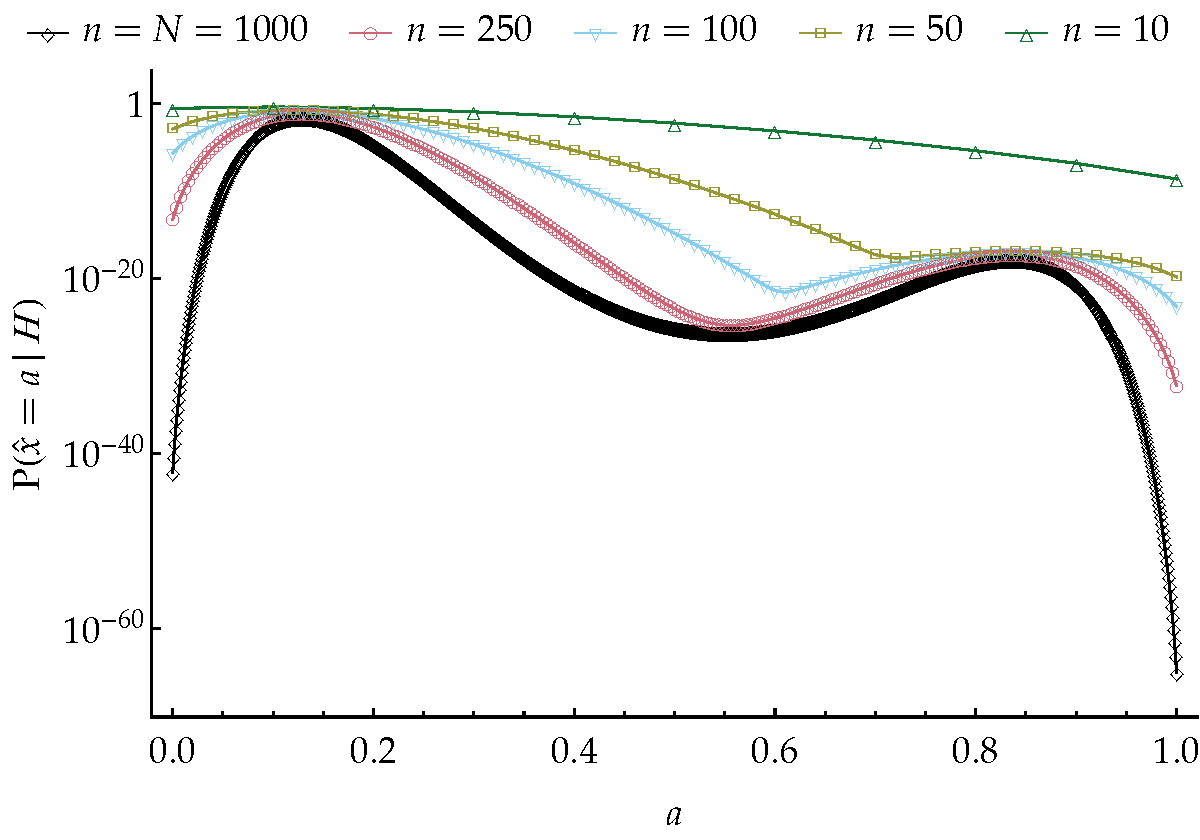
\includegraphics[width=0.95\columnwidth]{scaled_subpop_probs.pdf}%
\caption{Probability distributions $\p(\yxs = a \cond \yH)$ for different
  subnetwork sizes $n$, obtained from a network probability
  distribution $\p(\yXf = A \cond \yH)$ having the maximum-etropy
  form~\eqref{eq:full_pop_av_example_ME}.}
\label{scaling_distr}
\end{figure}
\begin{figure}[!p]
\centering
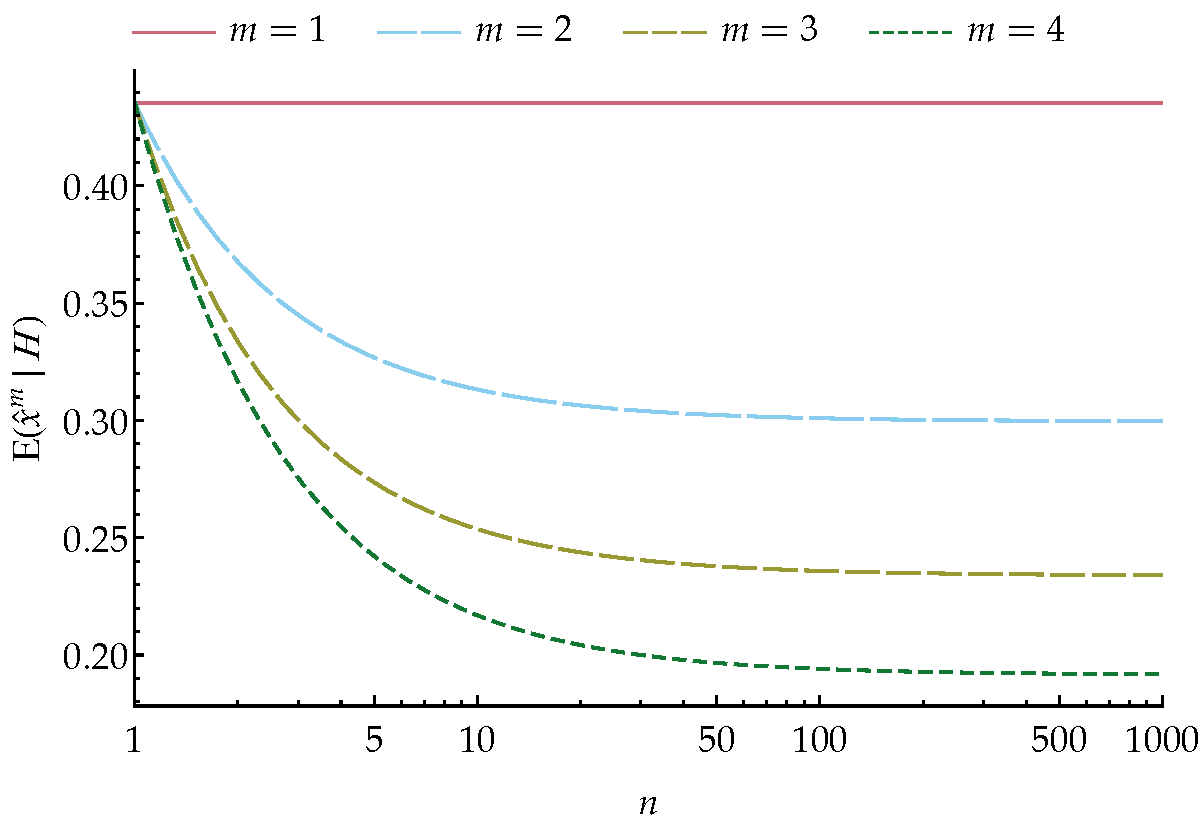
\includegraphics[width=0.95\columnwidth]{scaling_subpop_moments.pdf}%
\caption{Moments of the probability distributions $\p(\yxs =a \cond
  \yH)$ as functions of the subnetwork size $n$.}
\label{scaling_moments}
\end{figure}

The probability distribution of \eqn~\eqref{eq:full_pop_av_example_ME} is
plotted in \fig~\ref{scaling_distr}, together with the resulting
subnetwork-average distributions $\p(\yxs = a \cond\yH)$, for the case in
which $N = 1000$ units, $\lambda_1=-2.55$, $\lambda_2=0.005$, and
$n=10, 50, 100, 250$. The distributions become broader as $n$ decreases,
and the minimum of the original distribution disappears; at the same time
the finite-difference
\[\frac{\p(\yxs=a+1/n\cond\yH)-\p(\yxs=a\cond\yH)}{1/n}\]
presents a sharp jump at this minimum when $n\approx 100$.

To the eye familiar with maximum-entropy distributions, the
subnetwork-average distributions of \fig~\ref{scaling_distr} do not look
like maximum-entropy ones with second-moment constraints. In fact,
they are not and \emph{cannot} be:
\begin{equation}
  \label{eq:maxent_form_sub}
  \p(\yxs =a  \cond \yH)
\ne\kappa\binom{n}{n a}\exp[\yk_2\, n a\,(n a-1)/2 + \yk_1\, n a]
%\quad\text{(false)}
\end{equation}
for any $\kappa, \yk_1, \yk_2$, unless $n=2$. This impossibility holds more
generally for any number of constraints $m$ and subnetwork size $n$ such
that $m<n$. The reason is simple: suppose we have assigned a
maximum-entropy distribution with $m$ moment constraints as the
distribution for the network average. If we want the same kind of
distribution for a subnetwork of size $n$, we are free to play with $m+1$
parameters (normalization included), but we must also satisfy the $n+1$
equations corresponding to the marginalization~\eqref{eq:subpop_average}.
This is generally impossible unless $m \ge n$. (Impossibilities of a
similar kind appear in statistical mechanics, see \eg\
ref.~\citep{maesetal1999}.)
%file: test_ME_same_under_scaling.nb

This fact can be significant for recent works
\citep[\eg,][]{schneidmanetal2006,shlensetal2006,tkaciketal2006,marreetal2009,tkaciketal2009,ganmoretal2011,shimazakietal2012,tkaciketal2013,shimazakietal2015}
in which a maximum-entropy probability distribution with second- or
third-moment constraints is assigned to relatively small subnetworks
($n < 200$) of neurons. If we assume that such subnetwork is part of a
larger network, and assume the condition of symmetry~\eqref{eq:homog_math},
then the larger network \emph{cannot} be assigned a maximum-entropy
distribution with the same number of constraints. Vice versa, if we assign
such a maximum-entropy distribution to the larger network, then none of its
subnetwork of enough large size $n$ can be assigned a similar
maximum-entropy distribution. See ref.~\citep{rostamietal2016} for a
broader discussion of this fact and of its consequences.

\medskip

The dependence of the first four moments $\expe{\yxs^m \cond \yH}$ as a
function of size $n$ is shown in \fig~\ref{scaling_moments}. The moments
become practically constant when $n \approx 100$ or larger. The
expectations of $m$-tuple products of states
$\expe{x_{i_1}\dotsm x_{i_m} \cond \yH}$, proportional to the factorial
moments, are not shown as they do not depend on $n$.


\subsection{From subnetwork to network}
\label{sec:from_sub_to_full}

We have seen that, given the condition of symmetry~\eqref{eq:homog_math},
the probability $\p(\yXf = A \cond\yH)$ for the network average determines
that of each subnetwork average, $\p(\yxs \cond\yH)$, by the
marginalization \eqn~\eqref{eq:subpop_average}. The reverse is trivially
not true, since \eqn~\eqref{eq:subpop_average}, as a linear mapping from
$\RR^{N+1}$ to $\RR^{n+1}$, with $N$ larger than $n$, is onto but not into.
Assigning a probability distribution $\p(\yxs = a \cond\yH)$ to a
subnetwork average $\yxs$ does not determine a network distribution
$\p(\yXf = A\cond\yH)$: it only restricts the set of possible ones; this
set can in principle be determined via linear-programming methods
\citep{hailperin1965,hailperin1984,hailperin1996,hailperin2006,hailperin2011}.
\begin{innote}
  Analogous situations appear in the truth-valued logical calculus: if the
  composite proposition $\varAlpha\limplies \varBeta$ is assigned the
  truth-value \enquote{true}, then assigning $\varAlpha$ the value
  \enquote{true} also determines the value of $\varBeta$, whereas assigning
  $\varBeta$ the value \enquote{true} leaves the value of $\varAlpha$
  undetermined.
\end{innote}
The same linear-programming methods show that any inference from subnetwork
properties to network ones must necessarily start from some assumptions
$\varIota$ that assign a probability distribution
$\p(\yX = \yR \cond \varIota)$ for the network states. The approaches to
this task and reformulations of it have become uncountable: they include
exchangeable models, parametric and non-parametric models, hierarchical
models, general linear models, models via sufficiency, maximum-entropy
models, and whatnot
\citep[\eg:][]{jeffreys1931_r1973,jeffreys1939_r2003,jaynes1994_r2003,bernardoetal1994,gelmanetal1995_r2014,ghoshetal1997,kallenberg2005,gregory2005,sivia1996_r2006,ferreiraetal2007,dawid2013,damienetal2013}.
We now show two examples, based on a maximum-entropy approach, that to our
knowledge have not yet been explored in the neuroscientific literature. For
a concrete application see \citep{rostamietal2016b}.



\paragraph{First example: moment constraints for the network.}
\label{sec:maxent_moments}
Consider a state of knowledge $\yHa$ leading to the following properties:
\begin{enumerate}[$\yHa$1.]
\item the expectations of the single and pair averages $\yxs$ and
  $\sav{\yx\yx}$ of a particular subnetwork have given values
  \begin{equation}
    \label{eq:constr_ex1}
    \expe{\yxs \cond \yHa} = c_1, \qquad \expe{\sav{x_i x_j}\cond\yHa} = c_2;
  \end{equation}
\item the network probability distribution $\pr(\yX = \yR \cond\yHa)$
  has maximum relative entropy with respect to the uniform one, given the
  constraints above.
\end{enumerate}

\medskip Then the probability distribution for the network conditional on $\yHa$
is completely determined: it satisfies the symmetry
property~\eqref{eq:homog_math} and is defined by
\begin{multline}
  \label{eq:pop_distr_maxent1}
  \pf(\yX =\yR \cond\yHa) =
\varKappa\exp[\yL_2 N\yRf\,(N\yRf-1)/2 + \yL_1 N\yRf]
\\
\!\begin{aligned}[b]
&\text{with $\varKappa, \yL_m$, such that the distribution is normalized and}
\\
&\varKappa\sum_{N A=0}^N %m!\,
\binom{N-m}{N A-m}
\exp[\yL_2 N A\,(N A-1)/2 + \yL_1 N A]
= c_m, \quad m=1,2.
\end{aligned}
\end{multline}
We omit the full proof of this statement: it is a standard application of
the maximum-entropy procedure
\citep[\eg:][]{jaynes1957,jaynes1963,good1963,jaynes1967,jaynes1979b,vancampenhoutetal1981,sivia1990,fangetal1997,bretthorst2013},
combined with the equality~\eqref{eq:expe_products} of subnetwork and
network expectations, \eg
\begin{equation}
  \label{eq:exploit_eq_expects}
  c_2 = \expe{\sav{\yx\yx}\cond\yHa} =
\binom{N}{2}^{-1}
\sum_{N A=0}^N %m!\,
\binom{N A}{2} \, \p(\yXf = A\cond\yHa),
\end{equation}
and with relations~\eqref{eq:joint_plaus_N_homog},
\eqref{eq:conditional_total_state}. This example is easily generalized to
any number $m$ of constraints such that  $m\le n$.

Note again that, as remarked in \sect~\ref{sec:pop2sub_examples}, the
subnetwork from which the averages in the
expectations~\eqref{eq:constr_ex1} are calculated has a probability
distribution $\p(\yxs =a \cond\yH)$ determined by the
marginalization~\eqref{eq:subpop_average} and does \emph{not} have a
maximum-entropy form with the same number of constraints.
%file: test_ME_same_under_scaling.nb


\paragraph{Second example: subnetwork-distribution constraint.}
\label{sec:maxent_fullsubpop}
Consider another state of knowledge $\yHb$ leading to the following
properties:
\begin{asparaenum}[$\yHb$1.]
\item the average $\yxs$ of a particular
  subnetwork has a probability distribution $q$:
  \begin{equation}
    \label{eq:constr_subpop_distr}
    \pr(\yxs =a \cond\yHb) = q(a);
  \end{equation}
\item the probability distribution for the network, $\p(\yX = \yR
  \cond\yHb)$, has maximum relative entropy with respect to the uniform
  one, given the constraint above.
\end{asparaenum}

\medskip Then the probability distribution for the network given $\yHb$ is
completely determined and satisfies the symmetry
property~\eqref{eq:homog_math}:
\begin{multline}
  \label{eq:pop_distr_maxent2}
  \p(\yX= \yR \cond\yHb) =
\exp\Biggl[
\sum_{n a=0}^n \yL_{ a}
%\binom{N}{N\yXf}^{-1}
\binom{n}{n a}
\binom{N-n}{N\yRf-n a}\Biggr]
\\
\!\begin{aligned}[b]
&\text{with $\yL_{ a}$ such that}
\\
&\sum_{N A=0}^N
%\binom{N}{N A}^{-1}
\binom{n}{n a}
\binom{N-n}{N A-n a}\,
\exp\Biggl[
\sum_{n a=0}^n \yL_{ a}
%\binom{N}{N A}^{-1}
\binom{n}{n a}
\binom{N-n}{N A-n a}\Biggr]
=q( a)
\end{aligned}
\end{multline}
(the normalization constraint being unnecessary since $q$ is normalized).
This result is just another application of the maximum-entropy procedure
with $n+1$ (linear) constraints given by \eqn~\eqref{eq:marginal}, where
the left-hand side is now given and equal to $q(a)$.

This example is equivalent to the generalization of the previous one with
$n$ moment constraints, since knowledge of $\pr(\yxs=a \cond \yHb)$ is
equivalent to knowledge its first $n$ moments.

\bigskip

The above examples do not mention how the values of the expectation
constraints or of the subnetwork-average probability distribution can have
been assigned. They cannot be assigned by a measurement, of course, since
probabilities and expectations are not physical quantities and cannot be
physically measured -- they represent guesses of an observer and depend on
the observer's state of knowledge and assumptions. Rather, such values
usually come from measurements made on \enquote{copies} -- in a very
general sense -- of the states of the network; \eg, when we have a time
sequence of them and measure the frequencies of their occurrence. Such
situations can again be fully analysed with the probability calculus, and
one can show \citep{portamana2009} that the maximum-entropy formulae in the
examples above are just limit forms of such an analysis, employing
measured physical data $\varDelta$ like, \eg, frequencies, and
repeated applications of Bayes's theorem,
\begin{equation}
  \label{eq:bayes_thm}
  \p(\yX =\yR\cond \varDelta, \varIota) \propto
\p(\varDelta \cond \yX=\yR, \varIota)\, \p(\yX =\yR \cond \varIota),
\end{equation}
which updates the initial probability assignments on such data. But the
discussion of this is again outside the scope of this Note.





\bigskip

\section{On the  symmetry property}
\label{sec:stoch_symm}

The symmetry property~\eqref{eq:homog_math} is called \emph{finite
  exchangeability} in the Bayesian literature and, as was mentioned in
\sect~\ref{sec:main_formulae}, its relation to the hypergeometric
distribution in expression~\eqref{eq:subpop_average} for the subnetwork
average is
well-known
\citep{kendall1967,definetti1969b,heathetal1976,diaconis1977,diaconisetal1980,jaynes1986c}.


This property can reflect two very different states of knowledge:
either \begin{inparaenum}[(a)]\item knowledge that the network is somehow
  \emph{physically homogeneous}, or
\item \emph{complete ignorance} about the network's homogeneity or inhomogeneity.
\end{inparaenum}
In the second case we are saying that the indices or labels \enquote{$i$}
of the units are \emph{uninformative} -- because, for example, we have no
idea of how the units were labelled, hence we cannot presuppose any
relation among the units, nor can we presuppose any structural or
topological properties of the network they constitute. In the first case we
are saying that the labels are \emph{irrelevant}, even though they might be
informative. The reason could be that, even if there is a connection
between labels and, say, spatial locations of the units, each unit is
nevertheless physically, homogeneously, identically connected to all the
others; so we assume that spatial location does not play a relevant role.

An important consequence of the symmetry property is that no amount of new
evidence about an \emph{a}symmetry in the labelling of some units can lead
to asymmetric predictions about the remaining ones. For example, if we have
new data $\yD$ saying that the first $n$ units are in state $1$ and the
last $n$ in state $0$,
\begin{equation}
 \yD \defd (X_1 = X_2 = \dotsb = X_n =1,\quad
X_{N-(n-1)}= \dotsb = X_{N-1} = X_N = 0),
\end{equation}
with $n$ large, our updated probabily distribution will still assign (as
can be shown using \eqns~\eqref{eq:homog_math} and
\eqref{eq:joint_plaus_N_homog}) the same probability for their respective
neighbouring units with labels $n+1$ and $N-n$ to be in state $1$ or $0$:
\begin{equation}
  \label{eq:same_prob_symm}
  \begin{split}
  \p(X_{n+1} =1 \cond \yD,\yH) &= \p(X_{N-n} =1 \cond \yD,\yH),
  \\
  \p(X_{n+1} =0 \cond \yD,\yH) &= \p(X_{N-n} =0 \cond \yD,\yH).
\end{split}
\end{equation}
This may seem unreasonable -- we would now say that the unit $n+1$ is more
likely to be in state $1$, as the first $n$ are, than in $0$; and that the
unit $N-n$ is more likely in state $0$, as the last $n$ are, than in $1$;
\ie
\begin{equation}
  \label{eq:wished_result}
  \begin{split}
  \p(X_{n+1} = 1 \cond \yD,\yH) &>  \p(X_{n+1} = 0 \cond \yD,\yH),
\\
  \p(X_{N-n} = 1 \cond \yD,\yH) &<  \p(X_{N-n} = 0 \cond \yD,\yH),
\end{split}
\end{equation}
which is equivalent to $\p(X_{n+1} = 1 \cond \yD,\yH) > \tfrac{1}{2}$,
$\p(X_{N-n} = 1 \cond \yD,\yH) < \tfrac{1}{2}$; but the
equalities~\eqref{eq:same_prob_symm} make this impossible.

The two very different motivations behind the symmetry property -- lack of
information and lack of relevance -- can of course be handled differently
by the probability calculus, in such a way that the appearance of asymmetry
in new data leads to asymmetry in updated predictions. But this requires a
more complex set of assumptions than those embodied in $\yH$; it requires,
in particular, some sort of probability distribution for the degree of
physical symmetry or homogeneity of the network, appropriately quantified.

The moral is that we should use the symmetric assumption $\yH$ only if we
can safely exclude the presence of inhomogeneity or are uninterested in
detecting its presence. Otherwise, we must resort to more appropriate (and
complex) assumptions. If we repeatedly observe new values that happen to
have a very low probability according to the updated distribution
$\p(\yX = \yR \cond \yD_1,\yD_2,\dotsc, \yH)$, this could be an indication
that the symmetry property is unreasonable. Any strong departure of higher
powers of measured averages from their expected behaviour given in
\eqn~\eqref{eq:moments} and illustrated in \fig~\ref{scaling_moments} can
also be an indication that the symmetry property may have to be abandoned;
hence the usefulness of \eqn~\eqref{eq:moments}.





\section{Summary and remarks}
\label{sec:summary}

The main point of this Note was to explicitly collect and illustrate the
mathematical formulae \ref{item:tot_plaus}--\ref{item:moments},
\sect~\ref{sec:main_formulae}, between the probabilities assigned to the
state of a network of neurons (or similar entities), and those assigned to
the state of a subnetwork thereof. The formulae hold in the simple case of
binary states and under an assumption of symmetry. Such relations can be
found in several classical texts on probability and statistics; but we
deemed it useful to restate them in a neuroscientific context, given their
fundamental importance in relating a whole to its parts.

We have indeed seen that these formulae lead to straightforward but in some
cases unexpected consequences: \eg, if a network is assigned a
maximum-entropy probability distribution, then its subnetworks
\emph{cannot} be assigned a maximum-entropy distribution of the same form,
and vice versa. The formulae also readily suggest new ways of making
inferences or of formulating starting assumptions. Discussion of these points
is left to forthcoming works \citep{rostamietal2016,rostamietal2016b}.

We also hope to have given the readers a feeling of the agility and
simplicity with which the probability calculus (\enquote{Bayesian theory})
leads us from assumptions to consequences (albeit sometimes with non-simple
mathematics), and from consequences to the assessment of how suitable our
initial assumptions are, as shown with the assumption of symmetry.





\defbibnote{postnote}{\small\par\medskip\noindent{\footnotesize% Note:
\arxivp \mparcp \philscip \biorxivp}%
}

\newcommand{\citein}[2][]{\textnormal{\textcite[#1]{#2}}%\addtocategory{extras}{#2}
}
\newcommand{\citebi}[2][]{ref.\ \citep[#1]{#2}%\addtocategory{extras}{#2}
}
\newcommand{\subtitleproc}[1]{}

\printbibliography[postnote=postnote]












\end{document}
